\documentclass[aspectratio=169, 10pt]{beamer}

% ─── Theme & colours ─────────────────────────────────────────────────────────
\usetheme{Madrid}
\usecolortheme{default}
\definecolor{ATLASblue}{RGB}{0, 51, 102}
\definecolor{ATLASgold}{RGB}{200, 160, 0}
\setbeamercolor{structure}{fg=ATLASblue}
\setbeamercolor{frametitle}{bg=ATLASblue, fg=white}
\setbeamercolor{title}{bg=ATLASblue, fg=white}
\setbeamercolor{block title}{bg=ATLASblue!80, fg=white}
\setbeamercolor{block body}{bg=ATLASblue!8}
\setbeamercolor{alerted text}{fg=ATLASgold}
\setbeamerfont{frametitle}{size=\large, series=\bfseries}

% ─── Packages ────────────────────────────────────────────────────────────────
\usepackage[utf8]{inputenc}
\usepackage[T1]{fontenc}
\usepackage{amsmath}
\usepackage{booktabs}
\usepackage{tikz}
\usetikzlibrary{arrows.meta, positioning, shapes.geometric, fit}


% ─── Title ───────────────────────────────────────────────────────────────────
\title[GN2 Jet Flavour Tagging]%
      {\textbf{GN2: Transformer-Based Jet Flavour Tagging}\\
       \small A PyTorch Implementation}
\subtitle{Based on ATLAS Collaboration --- \textit{Nat.\ Commun.}\ \textbf{17}, 541 (2026)}
\author{}
\date{}

% ─── Footer ──────────────────────────────────────────────────────────────────
\setbeamertemplate{footline}{
  \leavevmode\hbox{%
    \begin{beamercolorbox}[wd=.5\paperwidth,ht=2.25ex,dp=1ex,center]{author in head/foot}%
      \usebeamerfont{author in head/foot}\insertshorttitle
    \end{beamercolorbox}%
    \begin{beamercolorbox}[wd=.5\paperwidth,ht=2.25ex,dp=1ex,right]{date in head/foot}%
      \usebeamerfont{date in head/foot}\insertframenumber{}/\inserttotalframenumber\hspace*{2ex}
    \end{beamercolorbox}}%
}
\setbeamertemplate{navigation symbols}{}

% ─────────────────────────────────────────────────────────────────────────────
\begin{document}

% ── Slide 1: Title ───────────────────────────────────────────────────────────
\begin{frame}
\titlepage
\vspace{-8pt}
\begin{center}
  \small
  \textbf{Goal:} train a transformer to classify jets from $p_p$ collisions
  as $b$, $c$, $\tau$, or light from raw tracking information
\end{center}
\end{frame}

% ── Slide 2: Motivation ──────────────────────────────────────────────────────
\begin{frame}{Why Jet Flavour Tagging?}
\begin{columns}[T]
  \begin{column}{0.55\textwidth}
    \begin{block}{Physics context}
      \begin{itemize}
        \item Jets are collimated sprays of hadrons --- the most abundant
              objects at the LHC
        \item Identifying the originating quark flavour is critical for:\\
              Higgs boson measurements ($H\to b\bar{b}$, $H\to c\bar{c}$),
              top quark physics, BSM searches
        \item $b$-hadrons live $\sim 1.5$~ps $\Rightarrow$ displaced secondary
              vertex detectable in the inner tracker
      \end{itemize}
    \end{block}
    \begin{block}{Four classes}
      \centering
      \vspace{2pt}
      \begin{tabular}{cl}
        \toprule
        Label & Jet type \\
        \midrule
        $b$ & contains a $b$-hadron \\
        $c$ & contains a $c$-hadron, no $b$ \\
        $\tau$ & hadronic $\tau$-lepton decay \\
        light & light quark or gluon \\
        \bottomrule
      \end{tabular}
      \vspace{2pt}
    \end{block}
  \end{column}
  \begin{column}{0.42\textwidth}
    \begin{block}{Previous approaches}
      \textbf{Two-stage pipeline:}
      \begin{enumerate}
        \item Low-level algorithms reconstruct displaced vertices from tracks
        \item High-level classifier (DL1d, Deep Neural Network) combines outputs
      \end{enumerate}
      \vspace{4pt}
      \textbf{GN2:} single end-to-end transformer --- no hand-crafted intermediate
      representations
    \end{block}
    \vspace{4pt}
    \begin{alertblock}{Key result (ATLAS)}
      At 70\% $b$-efficiency:\\
      $c$-jet rejection $\times 3.5$ better than DL1d\\
      light-jet rejection $\times 1.8$ better than DL1d
    \end{alertblock}
  \end{column}
\end{columns}
\end{frame}

% ── Slide 3: Dataset & Preprocessing ─────────────────────────────────────────
\begin{frame}{Dataset \& Preprocessing}
\begin{columns}[T]
  \begin{column}{0.48\textwidth}
    \begin{block}{Input data (HDF5)}
      \begin{itemize}
        \item Simulated ATLAS $t\bar{t}$ and $Z'$ events
        \item \textbf{Jet-level:} $p_T$, $\eta$
        \item \textbf{Track-level:} up to 40 tracks/jet\\
              impact parameters $d_0$, $z_0$, angular variables,
              quality flags
        \item \textbf{Label:} hadron PDG code $\to \{0,1,2,3\}$
      \end{itemize}
    \end{block}
    \begin{block}{Kinematic selection}
      $20 < p_T < 250$~GeV \quad $|\eta| < 2.5$\\[2pt]
      Stratified 70\,/\,15\,/\,15\% train/val/test split
    \end{block}
  \end{column}
  \begin{column}{0.48\textwidth}
    \begin{block}{Normalisation (\texttt{preprocess.py})}
      Computed on \textbf{training set only}:
      \begin{itemize}
        \item Jet $p_T$: log-transform $\to$ Z-score
        \item Jet $\eta$: Z-score
        \item Track variables: Z-score per feature
      \end{itemize}
      Saved to \texttt{norm\_stats.json} and reused at eval time
    \end{block}
    \begin{block}{Efficient I/O (\texttt{dataset.py})}
      \begin{itemize}
        \item Indices pre-sorted for \textbf{contiguous HDF5 reads}
        \item \texttt{\_BatchCollator}: single batched read per step
          vs. one read per sample
        \item Invalid tracks filtered via \texttt{"valid"} flag;
          remaining positions zero-padded with boolean mask
      \end{itemize}
    \end{block}
  \end{column}
\end{columns}
\end{frame}

% ── Slide 4: Architecture ─────────────────────────────────────────────────────
\begin{frame}{GN2 Architecture}
\begin{columns}[T]
  \begin{column}{0.52\textwidth}
    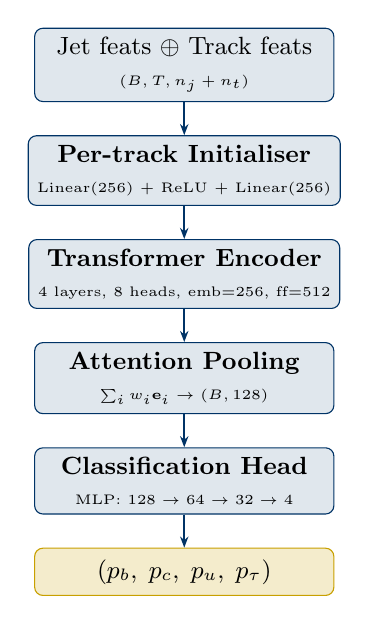
\begin{tikzpicture}[
        box/.style={rectangle, rounded corners=3pt, draw=ATLASblue,
                    fill=ATLASblue!12, minimum width=3.8cm, minimum height=0.6cm,
                    font=\small, align=center},
        arr/.style={-{Stealth[length=4pt]}, ATLASblue, thick},
        node distance=0.42cm
      ]
      \node[box] (inp) {Jet feats $\oplus$ Track feats\\
                        \tiny $(B,T,n_j+n_t)$};
      \node[box, below=of inp] (init) {\textbf{Per-track Initialiser}\\
                                       \tiny Linear(256) + ReLU + Linear(256)};
      \node[box, below=of init] (tf) {\textbf{Transformer Encoder}\\
                                       \tiny 4 layers, 8 heads, emb=256, ff=512};
      \node[box, below=of tf] (pool) {\textbf{Attention Pooling}\\
                                       \tiny $\sum_i w_i \mathbf{e}_i \to (B, 128)$};
      \node[box, below=of pool] (head) {\textbf{Classification Head}\\
                                         \tiny MLP: $128\to64\to32\to4$};
      \node[box, below=of head, fill=ATLASgold!20, draw=ATLASgold] (out)
            {$(p_b,\; p_c,\; p_u,\; p_\tau)$};
      \draw[arr] (inp) -- (init);
      \draw[arr] (init) -- (tf);
      \draw[arr] (tf) -- (pool);
      \draw[arr] (pool) -- (head);
      \draw[arr] (head) -- (out);
    \end{tikzpicture}
  \end{column}
  \begin{column}{0.45\textwidth}
    \begin{block}{Pre-LayerNorm Transformer layer}
      For each layer $\ell$:
      \[
        \mathbf{x}' = \mathbf{x} + \mathrm{MHA}(\mathrm{LN}(\mathbf{x}))
      \]
      \[
        \mathbf{x}'' = \mathbf{x}' + \mathrm{FFN}(\mathrm{LN}(\mathbf{x}'))
      \]
      Padding mask prevents attention to empty track slots.
    \end{block}
    \begin{block}{Attention pooling}
      \[
        w_i = \mathrm{softmax}\!\left(\mathbf{q}^\top \mathbf{e}_i\right),\quad
        \mathbf{g} = \sum_i w_i \mathbf{e}_i
      \]
      Pads masked to $-\infty$ before softmax.
    \end{block}
    \begin{alertblock}{}
      \centering $\sim$\,\textbf{2.3 M} trainable parameters\\
      ReLU activations throughout
    \end{alertblock}
  \end{column}
\end{columns}
\end{frame}

% ── Slide 5: Training ─────────────────────────────────────────────────────────
\begin{frame}{Training Pipeline}
\begin{columns}[T]
  \begin{column}{0.48\textwidth}
    \begin{block}{Loss function}
      Cross-entropy on 4 classes, labels $\{0,1,2,3\}$\\
      Jets with unmapped labels ($-1$) are ignored via
      \texttt{ignore\_index=-1}
      \[
        \mathcal{L} = -\sum_{i} y_i \log p_i
      \]
    \end{block}
    \begin{block}{Optimiser}
      \textbf{AdamW}, weight decay $\lambda = 10^{-5}$\\[3pt]
      \textbf{LR schedule:}
      \begin{enumerate}
        \item Linear warmup: $10^{-7} \to 5\times10^{-4}$ (first 1\% of steps)
        \item Cosine annealing: $5\times10^{-4} \to 10^{-5}$ (remaining steps)
      \end{enumerate}
    \end{block}
  \end{column}
  \begin{column}{0.48\textwidth}
    \begin{block}{Training details}
      \begin{itemize}
        \item Batch size: 1024 (configurable)
        \item Gradient clipping: $\|\nabla\|_\infty \le 1.0$
        \item Mixed precision (AMP) on CUDA
        \item Best checkpoint by validation loss
        \item TensorBoard logging
      \end{itemize}
    \end{block}
    \begin{block}{Code structure (\texttt{train.py})}
      \begin{itemize}
        \item \texttt{GN2Loss} --- loss module
        \item \texttt{lr\_scheduler()} --- warmup + cosine
        \item \texttt{run\_epoch()} --- single pass (train or val)
        \item \texttt{train()} --- full loop, returns best model
        \item \texttt{TrainingHistory} --- stores curves for plotting
      \end{itemize}
    \end{block}
  \end{column}
\end{columns}
\end{frame}

% ── Slide 6: Discriminants ────────────────────────────────────────────────────
\begin{frame}{Tagging Discriminants}
\begin{columns}[T]
  \begin{column}{0.48\textwidth}
    \begin{block}{$b$-tagging: discriminant $D_b$}
      \[
        D_b = \log\!\left(\frac{p_b}{f_c\,p_c + f_\tau\,p_\tau +
        (1-f_c-f_\tau)\,p_u}\right)
      \]
      \begin{itemize}
        \item $f_c = 0.2$, $f_\tau = 0.05$ (ATLAS defaults)
        \item $D_b > \text{threshold}$ $\Rightarrow$ jet is $b$-tagged
        \item Operating point (OP): value of threshold giving a target
              $b$-efficiency (e.g.\ 70\%)
      \end{itemize}
    \end{block}
  \end{column}
  \begin{column}{0.48\textwidth}
    \begin{block}{$c$-tagging: discriminant $D_c$}
      \[
        D_c = \log\!\left(\frac{p_c}{f_b\,p_b + f_\tau\,p_\tau +
        (1-f_b-f_\tau)\,p_u}\right)
      \]
      \begin{itemize}
        \item $f_b = 0.3$, $f_\tau = 0.01$ (ATLAS defaults)
        \item Same end-to-end model --- no retraining needed
      \end{itemize}
    \end{block}
  \end{column}
\end{columns}
\vspace{6pt}
\begin{block}{ROC curves (background rejection vs.\ signal efficiency)}
  For each background class $k$:
  \[
    \varepsilon_\text{sig}(\theta) = \frac{|\{D > \theta\} \cap \text{signal}|}{|\text{signal}|},
    \qquad
    R_k(\theta) = \frac{|\text{background}_k|}{|\{D > \theta\} \cap \text{background}_k|}
  \]
  Higher rejection at same efficiency = better tagger.
  Three curves per ROC plot: $c$-jet, light-jet, $\tau$-jet rejection vs.\ $b$-efficiency.
\end{block}
\end{frame}

% ── Slide 7: Evaluation Pipeline ─────────────────────────────────────────────
\begin{frame}{Evaluation Pipeline (\texttt{evaluate.py})}
\begin{columns}[T]
  \begin{column}{0.48\textwidth}
    \begin{block}{Outputs produced}
      \begin{enumerate}
        \item \texttt{metrics.json} --- accuracy, per-class P/R/F1
        \item \texttt{confusion\_matrix.pdf} --- normalised
        \item \texttt{score\_distributions.pdf} --- $p(c|$\,true flavour$)$
        \item \texttt{roc\_db.pdf} --- $b$-tagging ROC
        \item \texttt{roc\_dc.pdf} --- $c$-tagging ROC
      \end{enumerate}
    \end{block}
    \begin{block}{Usage}
      \ttfamily\footnotesize
      python -m transformer\_jet\_tagging.evaluate\\
      \hspace{1em}{-}{-}config configs/config.json\\
      \hspace{1em}{-}{-}device cuda
      \normalfont\normalsize\\[2pt]
      Checkpoint path and output dir read from config.
    \end{block}
  \end{column}
  \begin{column}{0.48\textwidth}
    \begin{block}{Inference flow}
      \begin{enumerate}
        \item Load best checkpoint with \texttt{GN2.from\_checkpoint()}
        \item Iterate test loader, collect softmax probabilities
        \item Drop jets with label $= -1$ (unmapped)
        \item Compute metrics with \texttt{scikit-learn}
        \item Compute $D_b$, $D_c$ and scan thresholds for ROC
        \item Save all figures (ATLAS style via \texttt{mplhep})
      \end{enumerate}
    \end{block}
    \begin{alertblock}{Results}
      \centering
      \textit{[To be filled after training]}
    \end{alertblock}
  \end{column}
\end{columns}
\end{frame}

% ── Slide 8: Full Pipeline Summary ───────────────────────────────────────────
\begin{frame}{Full Pipeline at a Glance}
\begin{center}
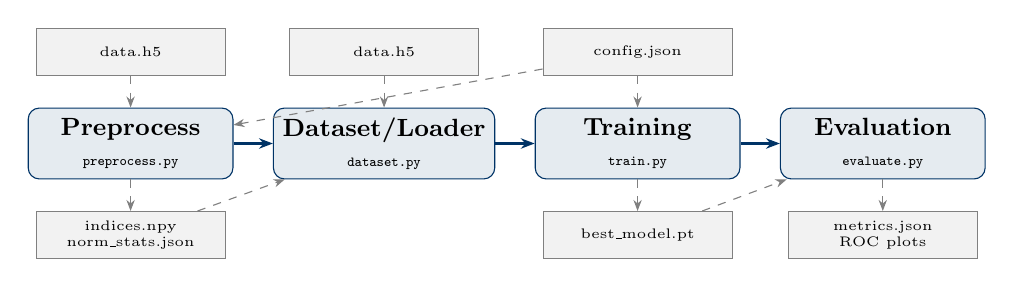
\begin{tikzpicture}[
    node distance=0.9cm and 0.5cm,
    box/.style={rectangle, rounded corners=4pt, draw=ATLASblue, fill=ATLASblue!10,
                minimum width=2.6cm, minimum height=0.9cm, align=center, font=\small},
    file/.style={rectangle, draw=gray, fill=gray!10, minimum width=2.4cm,
                 minimum height=0.6cm, align=center, font=\tiny},
    arr/.style={-{Stealth[length=5pt]}, ATLASblue, thick},
    garr/.style={-{Stealth[length=4pt]}, gray, dashed}
  ]
  \node[box] (pre) {\textbf{Preprocess}\\{\tiny \texttt{preprocess.py}}};
  \node[box, right=of pre] (ds) {\textbf{Dataset/Loader}\\{\tiny \texttt{dataset.py}}};
  \node[box, right=of ds] (tr) {\textbf{Training}\\{\tiny \texttt{train.py}}};
  \node[box, right=of tr] (ev) {\textbf{Evaluation}\\{\tiny \texttt{evaluate.py}}};

  \node[file, below=0.4cm of pre] (idx) {indices.npy\\norm\_stats.json};
  \node[file, below=0.4cm of tr]  (ckpt) {best\_model.pt};
  \node[file, below=0.4cm of ev]  (out) {metrics.json\\ROC plots};

  \draw[arr] (pre) -- (ds);
  \draw[arr] (ds) -- (tr);
  \draw[arr] (tr) -- (ev);
  \draw[garr] (pre) -- (idx);
  \draw[garr] (idx) -- (ds);
  \draw[garr] (tr) -- (ckpt);
  \draw[garr] (ckpt) -- (ev);
  \draw[garr] (ev) -- (out);

  % HDF5 input arrow
  \node[file, above=0.4cm of pre] (h5) {data.h5};
  \draw[garr] (h5) -- (pre);
  \node[file, above=0.4cm of ds] (h5b) {data.h5};
  \draw[garr] (h5b) -- (ds);

  % Config
  \node[file, above=0.4cm of tr] (cfg) {config.json};
  \draw[garr] (cfg) -- (pre);
  \draw[garr] (cfg) -- (tr);
\end{tikzpicture}
\end{center}

\vspace{4pt}
\begin{columns}
  \begin{column}{0.32\textwidth}
    \begin{block}{\small \texttt{preprocess.py}}
      \footnotesize
      Run once. Saves indices and normalisation stats.
    \end{block}
  \end{column}
  \begin{column}{0.32\textwidth}
    \begin{block}{\small \texttt{dataset.py}}
      \footnotesize
      Lazy HDF5 loading, batched reads, masking.
    \end{block}
  \end{column}
  \begin{column}{0.32\textwidth}
    \begin{block}{\small \texttt{train.py} / \texttt{evaluate.py}}
      \footnotesize
      Full training loop + test-set evaluation.
    \end{block}
  \end{column}
\end{columns}
\end{frame}

% ── Slide 9: Comparison with ATLAS GN2 ───────────────────────────────────────
\begin{frame}{Comparison: This Implementation vs.\ ATLAS GN2}
\begin{center}
\begin{tabular}{lll}
  \toprule
  \textbf{Aspect} & \textbf{ATLAS GN2} & \textbf{This implementation} \\
  \midrule
  Framework & PyTorch Lightning & PyTorch (plain) \\
  Architecture & Transformer + 2 aux.\ heads & Transformer (primary head only) \\
  Aux.\ objectives & Track origin + vertex grouping & \alert{Not implemented} \\
  Training data & $\sim\!200$M jets, 4 folds & Configurable subset \\
  Batch size & 12\,000 & 1024 (configurable) \\
  Hardware & NVIDIA A100 ($\sim$300 GPU-h) & Any CUDA/CPU device \\
  Input tracks & 40 (sorted by $|d_0/\sigma_{d_0}|$) & 40 (sorted by validity) \\
  LR schedule & Warmup + cosine & \checkmark\ Identical \\
  Deployment & ONNX Runtime & Checkpoint (.pt) \\
  \bottomrule
\end{tabular}
\end{center}
\vspace{4pt}
\begin{alertblock}{Main limitation}
  The two \textbf{auxiliary training objectives} (track origin classification
  and track-pair vertex grouping) are not included.
  These contribute up to 30\% improvement in background rejection according to
  the ATLAS paper and are the main target for future extensions.
\end{alertblock}
\end{frame}

% ── Slide 10: Summary & Next Steps ───────────────────────────────────────────
\begin{frame}{Summary \& Next Steps}
\begin{columns}[T]
  \begin{column}{0.48\textwidth}
    \begin{block}{What has been implemented}
      \begin{itemize}
        \item[$\checkmark$] End-to-end GN2 architecture (transformer + pooling)
        \item[$\checkmark$] Optimised HDF5 data pipeline with batched reads
        \item[$\checkmark$] Preprocessing with data-leakage-free normalisation
        \item[$\checkmark$] Training: AdamW + warmup/cosine LR, AMP, early stopping
        \item[$\checkmark$] Evaluation: metrics, confusion matrix, ROC curves
        \item[$\checkmark$] Configurable via JSON; all modules standalone-runnable
      \end{itemize}
    \end{block}
  \end{column}
  \begin{column}{0.48\textwidth}
    \begin{block}{Known issues to fix}
      \begin{itemize}
        \item Bug in \texttt{preprocess.py}: double-nested \texttt{data\_config["data"]}
        \item \texttt{constants.py} / \texttt{\_\_init\_\_.py} to be verified
        \item \texttt{label\_map} inversion in \texttt{evaluate.py}
      \end{itemize}
    \end{block}
    \begin{block}{Future extensions}
      \begin{itemize}
        \item \textbf{Auxiliary objectives}: track origin + vertex grouping
              ($\to$ up to 30\% rejection gain)
        \item \texttt{efficiency\_at\_wp()} for working-point tables
        \item \texttt{pyproject.toml} and \texttt{tests/} directory
        \item 4-fold cross-training (ATLAS production strategy)
        \item ONNX export for deployment
      \end{itemize}
    \end{block}
  \end{column}
\end{columns}
\vspace{4pt}
\begin{center}
  \small\color{gray}
  Reference: ATLAS Collaboration, \textit{Nature Communications} \textbf{17}, 541 (2026)
  \quad|\quad
  Training code: \texttt{salt} (JOSS, 2025)
\end{center}
\end{frame}

\end{document}